%-------------------------------------------------------------------
\chapter{Methods}
\label{ch:methods}
%-------------------------------------------------------------------

\epigraph{\enquote{The illusion that we understand the past fosters overconfidence in our ability to predict the future.}}{\emph{Daniel Kanheman}}

\section{Limits of XAI}
\label{sec:limits of XAI}
In the fields of philosophy, psychology and cognitive science there are a lot of mature works addressing the problem of what an explanation is and how people evaluate its quality, but most of eXplainable Artificial Intelligence (XAI) research is based on an intuitive idea of what constitutes a “good” explanation because seeking explanations as defined by such social sciences would lead to failure~\cite{Miller}.
There is an \textit{Explanatory Gap} (EG) between natural language and mathematical language expressiveness which undermines the possibility of rigorously defining what an explanation is in mathematical terms, necessary for applying it to artificial intelligence systems.
Hence, research in the field of XAI is driven by mathematical heuristics that result in intuitively “good” explanations.
However, humans are known to be highly biased when taking their decisions intuitively rather than through critical analysis~\cite{Kahneman}. 

To show how humans are not good at intuitively judging what a good explanation is, consider for instance the family of XAI post-hoc methods in computer vision that produce a saliency map (a.k.a. heat map) as explanation (e.g. GradCAM~\cite{GradCAM}).
They are so-called local methods, meaning: given an input image $\mathbf{I}$ and a model $f$, they return an explanation of its specific prediction $y = f(\mathbf{I})$.
This explanation is a map assigning an “importance” score to image pixels.
It is easily visualizable (usually overlaid on the input image $\mathbf{I}$, see figure~\ref{fig:grad_cam}) by a human who, by visual inspection, can immediately grasp which parts of the image are supposedly more relevant for that prediction by $f$.

\begin{figure}
    \centering
    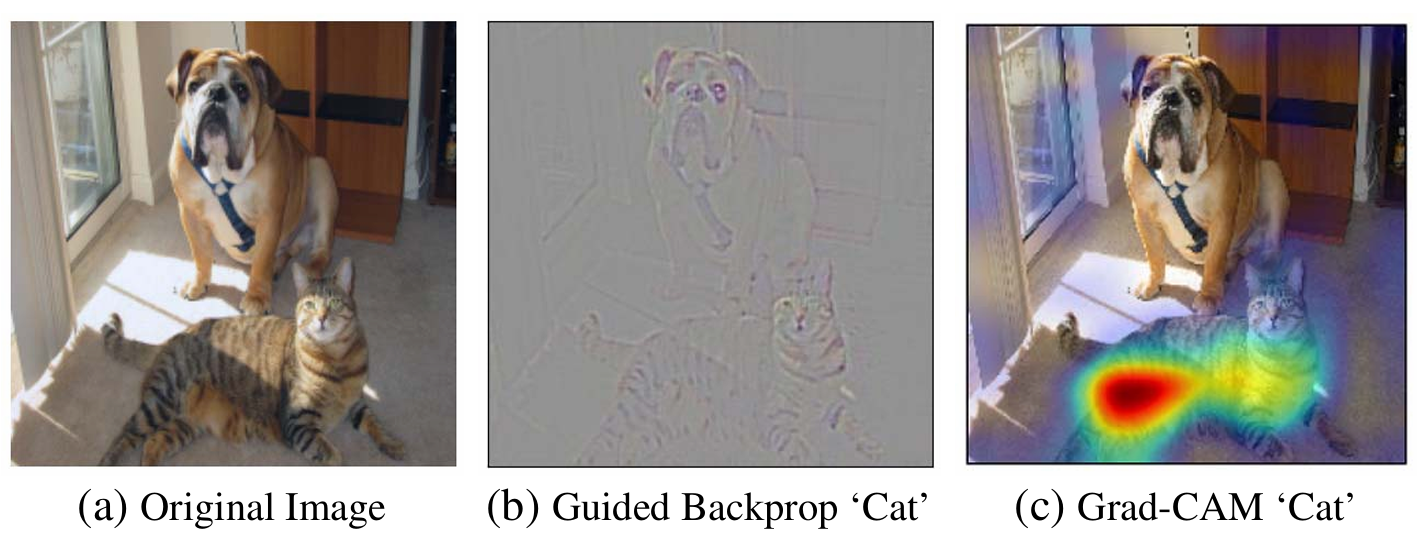
\includegraphics[width=0.8\textwidth]{figs/grad_cam}
    \caption{
        Image from~\cite{GradCAM}.
        (a) Original image.
        (b) Saliency map obtained with another method.
        (c) Saliency map (with respect to the class "cat") obtained with GradCAM and overlaid onto the original image.
        \label{fig:grad_cam}
    }
\end{figure}

For example if the model solves a classification problem then the highlighted pixels represent “where it looked at” for taking the classification decision.
However, the explanatory gap of above is filled by human cognition.
Indeed, humans perceive images at first sight in a very rich way and decompose it directly into objects, materials, lights, shadows, reflections, geometry~\cite{pinker2009mind}.
This implies that when looking at an image with highlighted areas (as it is when visualizing a saliency map) it is difficult to separate the rich conscious experience of the image from the actual information provided by the explanation.
The explanation has a very specific mathematical meaning, but it will look “good” as long as the highlighted area roughly contains reasonable parts of the image involved in humanly justifying the ground truth answer.
For instance, the model classifies an image as a cat and cat pixels are highlighted.
Although this kind of explanation is informative of the model behavior and can be effectively used for debugging purposes \cite{molnar2022}, it doesn't increase its interpretability.
It doesn't inform about how the model took its decision but rather which was it. 

All XAI methods suffer from similar problems: they provide seemingly “good” explanations, which appear so because of cognitive biases, but don't actually increase interpretability of the model on which they are applied because of the specific mathematical meaning of their explanations.
This is a consequence of the EG which limits human understanding of complex mathematical artificial intelligence models.
This can be alleviated by making assumptions about the targeted task.
The more assumptions are made when developing a model, the smaller the gap is.
In fact assumptions simplify reality, making it more easily representable in mathematical terms and leading to a better understanding of the resulting AI model.

This kind of flaws can be found also in the methods discussed in section~\ref{sec:SIDE and interpretability}.

\vspace{0.5cm}

Let's start from the work of You~et~al.~\cite{towards_interpretable}.
The authors assume that \textit{depth selectivity} of feature channels is a measure of interpretability without explaining why.
They rather give general analogies with other works where a similar dissection of the network behavior was done but for different tasks.
The proposed interpretability measure is arguably a bad measure.
Consider a \textit{bin} depth estimation method (refer to section~\ref{sec:bin_methods} for examples).
In such methods there are usually "bin discriminating layers" (BDLs) that are specialized in classifying input pixels with a bin label through the activation of a feature map.
Depth selectivity measures how much some layers of the model work like a BDL, so for instance a bin method in correspondence of BDLs would appear to be highly interpretable.
But BDLs are the second-to-last step in depth estimation based on bin methods, where the last is just an aggregation of the bin scores into a depth value.
Hence, for You et al., an interpretable network that performs depth estimation is just a network that solves the task in early layers, i.e. a smaller network.

\vspace{0.5cm}

In "Visualization of Convolutional Neural Networks for Monocular Depth Estimation"~\cite{Hu}, Hu~et~al. are biased in defining their explainability method (in this case a saliency method).
They repeatedly notice that if the mask $\textbf{M}$ is not properly optimized the result will be "unexpected" or not "useful".
So, while other formulations of the optimization problem defining such a mask are mathematically equivalent, the regularization is chosen based on the resulting appearance.
Hence, the authors are biased in picking up the explanation that satisfy their expectations about how it should look like.
Notice that their objective is \textit{not} to output a good-looking image, but to investigate the behavior of the model.
While their visualization method can be useful, it is based on an arbitrary concept of "relevance" for pixels contributing to the prediction.

\vspace{0.5cm}

The first work discussed in section~\ref{sec:SIDE and interpretability}, from Dijk~et~al.~\cite{Dijk}, sheds light on various potential biases of models trained on the KITTI dataset.
It is not meant to \textit{explain} their behavior, but it is informative nonetheless and uses valid methods for investigating models, that is: altering input images and looking for correlations in the resulting depth maps.
The main problem, related to what was discussed in this section, is about how the authors linguistically frame their results.
In fact, the probed model is said to "detect changes in the camera pitch", "recognize objects" and "rely on vertical position of objects".
While this way of expressing the results of the experiments is a useful abstraction, it risks attributing capabilities to the model that it does not have.
Humans are biased.
Consider a model given an image depicting a car as input.
Assume that the shape of the car is present in the predicted depth map.
When looking at it, it is immediate to say that the model \textit{recognized} the car.
What does it mean for an algorithm to "recognize an object" in an image?
Is the shape of a car present in the depth map because the network "recognized the car" or because of something else?
Natural language describing numerical results can be misleading, unfortunately expressing results in this way is a common practice in the field of XAI.

\vspace{0.5cm}

\section{Limits of Interpretability}
\label{sec:limits of interpretability}

In the previous section the concept of \textit{Explanatory Gap} (EG) was introduced.
The EG refers to the impossibility of mathematically defining what an explanation is because the richness of human language, psychology and cognition, that define what an explanation is for humans, is not captured by formal languages.
From now on, "explanatory gap" will more generally refer to the discrepancy between natural language and mathematical language expressiveness, which consequences go beyond the field of XAI.
In fact, this same gap is also the reason for which training objectives expressed as mathematical functions do not account for the complexity of real-life goals involved in tasks such as driving~\cite{Zablocki2022}.
Another example is in section~\ref{sec:metrics} where it was observed that satisfying metrics for depth estimation are yet to be found.

The EG has important consequences on interpretability of algorithms.
In order to clarify this point, consider that, when designing an algorithm for solving a certain problem, a developer represents the entities relevant to the problem and relations between them into mathematical language.
Since the natural language is more expressive than mathematical one, it could happen that some concepts cannot be faithfully translated into mathematical representations.
The transparency of an algorithm (concept introduced in section \ref{sec:deep learning and interpretability}) comes from the human understanding of its passages which are supposed to represent meaningful operations.

Entities and relations are represented in form of data structures and functions.
Computations and data manipulations can alter the meaning of such representations.
For instance, if a variable contains a positive real number that represents a distance, storing a negative value in it does not preserve its representation.
Ideally, in each step of an algorithm it should be possible to interpret what's happening by referring to what variables and functions represent.
In a neural network this is hardly possible since only its input and its output represent something meaningful to humans and what's in between is left to be learned by the model during training.
Theoretically, if extensive studies are performed on a specific model with fixed weights, a more in-depth understanding is possible, but it is an expensive process that, to my knowledge, no one has yet accomplished.
Researchers only have general ideas of what intermediate feature maps represent and don't analyze a single instance of a model, rather the focus is on a class of models defined by a certain architecture.
Deep learning is mainly used in tasks that are difficult to tackle via a formal and interpretable approach.

In fact, a task involving high-level human requests or concepts impossible to mathematically represent, requires an algorithm solving it to \textit{not} preserve representations.
This results in algorithmic steps that do not have a meaning.
It can be concluded that such tasks will always have a certain degree of non interpretability.
This has a fundamental consequence on the whole field of XAI: interpretability methods cannot return arbitrarily good explanations for algorithms solving such tasks.
Most importantly: there is an upper limit to intrinsic interpretability (transparency) of algorithms dependent on the task they solve.

\vspace{0.5cm}

Not all tasks are affected in the same way by this fact.

Formal tasks (e.g. sorting an array or searching in a graph) are not affected at all.
They are naturally expressed in mathematical terms and formal language is sufficient for solving eventual ambiguities.
Their solutions are completely understood and interpretable as they are justified by formal proofs or by rigorous arguments.

The most susceptible tasks to the explanatory gap are those that require imitating aspects of human cognition or linguistic abilities.
Examples are object detection, image segmentation, question answering, speech-to-text, driving.
This kind of tasks, here called \textit{human tasks}, cannot be tackled with a pure formal approach and needs semantic knowledge of the (perceived) world.
Because it's difficult to abstract from their own cognition, when dealing with such tasks humans are more easily biased.
Also, simplifying the problem by making assumptions is hardly ever possible, hence the formal approach is not viable.

Finally, there are tasks that deal with poorly understood parts of reality.
It is not clear how the EG affects them.
Examples are: predicting financial market prices or processing data coming from cutting-edge physics experiments.
Usually, experts apply both mathematical models (for instance the Black-Scholes model in finance) and black-box techniques when approaching them.
Since human knowledge is limited for these tasks (by definition), whether the latter techniques are necessary (implying a degree of intrinsic non-interpretability) or not is yet to be discovered.

\section{Interpretability of Depth Estimation}
\label{sec:interpretability of depth estimation}

\paragraph{Question.}
Depth estimation could be formally stated as the task of computing for a given image $\mathbf{I}$ its depth map $\mathbf{Z}$.
Can this problem be mathematically solved so that limitations of the EG do not apply?
Is depth estimation a human task?

\vspace{0.5cm}

\paragraph{Discussion.}
An image is the result of an image formation process which involves photons hitting a camera that measures their wavelength.
Photons coming from different directions contribute to determining the color of a pixel, but there is one direction in particular that contributes more.
A photon could bounce and be deviated before ending up traveling along such direction.
Eventually the photon will hit a camera photo-cell and participate in image formation.
The point in space where the photon was last deviated is associated to the pixel corresponding to the photo-cell.
Ideally, the $Z$ coordinate of such a point is the depth value of that pixel in the desired (metric) depth map.

The resulting image can be displayed using monitors, devices that can emit photons from a grid of photo-emissive elements.
While the image formation process is noisy, the displayed image will appear neat.
The reason for this is that the human brain cleans the information it receives.
Reality is noisy, vision deals with such noise continuously.
Through human perception, pixels are perceptually aggregated and form uniform visual units.
In this phase, many pixels are perceptually associated to different points in space other than those determined above.

The \textit{desired} depth map is hence defined by human visual perception that solves semantic ambiguities in the input signal, rather than by a well-defined physical process.
This implies that depth estimation (in the wild) is neither solvable nor definable using only mathematical language and reasoning.

\vspace{0.5cm}

If assumptions about images are made and the problem is formulated in the multi-view setting, it can be approached mathematically for the most part of it.
In the binocular setting, two images captured from different view-angles are used for estimating geometry of the scene under the form of disparity maps.
Epipolar geometry~\cite{multiview} studies the geometrical constraints of images capturing the same scene from different perspectives.
It can be used for determining depth values of corresponding pixels between the two views.
The problem is then reduced to finding these correspondences, since the rest is a mathematical and well-known reconstruction.

As stated, assumptions are needed for reducing to the minimum semantic ambiguities.
Surfaces in the scene should appear in the same way from different perspectives, i.e. be Lambertian surfaces.
For instance, a mirror appears differently based on what's reflecting.
Transparent materials exhibit a similar problem.
For successfully determining correspondences between the views, occlusion should be minimum and happen as distant from the camera as possible, otherwise it will invalidate a lot of pixels.
Another relevant factor is high frequency textures which make it impossible to successfully match pixels from different images belonging the same region in space.

\vspace{0.5cm}

Monocular depth estimation (MDE) is by no means solvable using only mathematical reasoning.
In fact, estimating a depth map from a single image is an ill-posed problem.
It is not possible to infer geometrical information about which path photon traveled from a single image, thus scene geometry is to be guessed by observing visual cues.
Human semantic knowledge (based on binocular viewing experience) solve visual ambiguities and produce a perception of depth.

Is human depth perception relevant in machine depth estimation?
Ground truth data is acquired using physical sensors or by rendering depth maps in graphical engines, hence it could be argued that humans have nothing to do with the task.
This would be a fallacy since ground truth data is pre-processed by human experts before resulting in ground truth depth maps.
Also, ground truth depth maps are usually incomplete (either sparse or with holes in them) and researchers have preferences on how MDE models should perform where the ground truth information is missing.
Finally, graphical engines are based on how humans organize physical reality and rendering algorithms are optimized to output photorealistic (i.e. as close to how humans visually perceive reality as possible) images based on simplified physical processes.

\vspace{0.5cm}

While it is difficult for humans to give accurate metric estimates of distances (and hence of depth), relative distance values can be estimated.
In creating the DIW dataset \cite{DIW}, people were asked to tell which pixel was closer to the camera given another through a crowd-sourcing process.
More accurate \textit{dense} relative depth maps could be estimated with software aided image measurements.
If such measurements are performed in stereo images or across video frames, metric depth estimation is feasible.
It is possible also to generate digital versions of real world scenes.
Artists can 3D model objects and reproduce environments.
Assisted by software that renders the digital scene and compares it with the reference image it could be possible to perform a precise depth annotation.
This further supports the claim that depth estimation is not a purely mathematical task and is about imitating human cognition and perception of the world.

\vspace{0.5cm}

\paragraph{Conclusion and implications.}
It can be concluded that \textit{MDE is a human task}.
This implies that monocular depth estimation methods present an intrinsic upper limit to their interpretability, as argued in the previous section.
This undermines the possibility of developing a fully interpretable algorithmic MDE.
A non-interpretable technique \textit{must} be employed by a method that solves such a task.

%\section{Evolutionary perspective}
%Artificial Intelligence (AI) is about producing algorithms that can compete with human intelligence in solving certain tasks.
%While it outperforms humans in specific tasks (like playing chess), it is not able yet to solve general tasks (e.g. driving a car).
%Humans cognitive capabilities are the result of billions of years of evolution.
%AI research is trying to beat the byproducts of evolution.
%I argue that evolution cannot be beaten and that a different approach is required in AI research.
%I will base my arguments on a simple model of evolution, found also in the field of evolutionary computing.
%
%A species can be modeled as a population of instances of a certain neural architecture.
%Each individual has its own network initialization and goes through a training phase (youth) and an evaluation phase (mature age).
%Each generation of individuals create its offspring.
%Newborn individual can present modification in the architecture topology.
%Only a percentage of individuals reproduce and the better they perform, the more likely are to reproduce.
%Parents can teach their offspring.
%During their lives, individuals gather data from the world and train on them.
%By educating their children, parents transmit relevant knowledge they acquired.
%
%Under this model, evolution is a massive Neural Architecture Search (NAS) performed for millions of years onto the human species.
%Even with the advent of new technologies, it's unlikely that better solutions than those found by evolution can be found by humans.
%In a recent paper \cite{udandarao2024zeroshotexponentialdatapretraining} (quoting the authors) it was found that, far from exhibiting "zero-shot" generalization, multimodal models require exponentially more data to achieve linear improvements in downstream "zero-shot" performance, following a sample inefficient log-linear scaling trend.
%This supports the idea that data will never be enough.

\section{Hybrid Approach to Depth Estimation}
\label{sec:hybrid}
In section~\ref{sec:interpretability of depth estimation} it was shown that non-interpretable techniques are \textit{necessary} for tackling monocular depth estimation (MDE).
State of the art methods developed in last years prove that a black-box model is also \textit{sufficient} for solving MDE.
The theoretical limitations of interpretability discussed in this chapter imply an \textit{upper limit} to transparency, not complete absence of it.
In order to achieve the maximal degree of interpretability for MDE methods, non-interpretable techniques need to be confined to some sub-tasks so that an interpretable pipeline can be built on top of them.
The objective is to reduce to the minimum the responsibilities of black-box models in the pipeline.
This would make it easier to build trust in the resulting hybrid method and increase its transparency to the theorized upper limit.

\vspace{0.5cm}

\paragraph{Learning problem.}
Given the set $\mathcal{I}$ of images and the set $\mathcal{Z}$ of depth maps, a probability distribution $\mathcal{D}$ is defined on $\mathcal{I} \times \mathcal{Z}$.

$\mathcal{D}$ specifies which input-output pairs are relevant for the task of MDE.
$\mathcal{I}$ is defined by the set of tensors valued in $[0, 1]$ and of various shape (assuming MDE is not constrained to a fixed image resolution).
The majority of these tensors do not define meaningful images.
Precisely, ignoring noisy oscillations, interesting images (where "interesting" is defined by $\mathcal{D}$) live in a low-dimensional manifold of the space of images $\mathcal{I}$.
An interesting image is still interesting if some noise is added to it.
Noise gives some "thickness" to the interesting image manifold, since it can go in any direction of the space as long as it has a negligible magnitude.
For simplicity, this fact about noise will be ignored throughout the discussion.

A loss function $\mathcal{L}: \, \mathcal{Z} \times \mathcal{Z} \rightarrow \mathbb{R}^{+}$ is defined on pairs of depth maps.
A learning problem is defined by a (large) \textit{finite} set $S$ of sampled input-output pairs from $\mathcal{D}$ and a loss function $\mathcal{L}$.
To solve the learning problem means to identify a set of functions $\mathcal{H}$ called "hypothesis space" \cite{ML_book} that realize the mapping $\mathcal{I} \rightarrow \mathcal{Z}$ and pick up a function $f \in \mathcal{H}$ that minimizes the expected value of $\mathcal{L}$ over $\mathcal{D}$:
\[
    \mathop{\text{argmin}}_{f \in \mathcal{H}} \, \mathbb{E}_{(\mathbf{I}, \, \mathbf{Z}) \sim \mathcal{D}} \, \mathcal{L}(f(\mathbf{I}), \, \mathbf{Z})
\]
The exact solution is usually impossible to find or to prove that it was found.
Heuristics are employed for choosing a good-enough solution $f \in \mathcal{H}$.
The process of choosing $f$ is called \textit{training} and consists in solving an optimization problem on $S$ that involves a simplified objective and some additional constraints that should improve the found solution (regularization terms).
In practice, the loss function used during training does not match the one to be globally minimized, called "error metric" $\mathcal{M}$ ("accuracy metric" if the problem is framed in terms of maximization).
In fact, it is common that metrics are non-differentiable, which makes it difficult to directly optimize them in particular when using a deep learning approach. 
Also, many metrics can be used for assessing the performance of solutions to complex task like MDE.
This is due to the complexity of the problem that cannot be captured by a single numerical measure, resulting in a multi-objective optimization problem.

%Under strong assumptions, theorems about solving learning problems have been proved (see \cite{ML_book}) that express limitations of the learned solution and characterize some properties of learning problems.
Relevant to this thesis is the fact that one can simplify the learning problem by changing $\mathcal{D}$, $\mathcal{L}$ or $\mathcal{H}$ and, doing so, increase the obtained performance measured by $\mathcal{M}$. 
The objective is to reduce the responsibilities of a trained black-box model in the MDE pipeline, leaving space for interpretable procedures.
For achieving this, a simplification of its defining learning problem is necessary.

\vspace{0.5cm}

\paragraph{Hybrid pipeline.}
The MDE task can be decomposed into the following sub-tasks: (1) estimate depth maps of image patches and (2) merge them into a full prediction.
This is common in the so-called "tile based" approach.
%An end-to-end neural architecture that frames MDE like this is PatchFusion~\cite{PatchFusion} and was discussed in subsection~\ref{subsec:patchfusion}.
To the purpose of defining a hybrid pipeline that increases the overall interpretability of the method, non-interpretable components should be confined to one sub-task only.
Since depth estimation was discussed to need a black-box approach to be solved, the first sub-task will be targeted with a (deep) learning approach.

Objective of this section is to simplify the learning problem to be solved in the first sub-task as much as possible.
In order to achieve this, patches cannot be too small since depth can be successfully estimated only if some global information is provided.
On the contrary, patches too large make the merging phase not necessary and the whole pipeline would reduce to a non-interpretable black-box prediction.
It is thus chosen that all patches must have the same shape $h \times w \times 3$, sufficiently smaller than the input image tensor $\mathbf{I}$ of shape $H \times W \times 3$.

Three modifications to the learning problem are proposed: to work with a subset of the possible patches, to pre-process them in the training phase and to change the optimization objective.
The second sub-task, namely to stitch together the partial depth predictions, is discussed in the next section.

\vspace{0.5cm}

\paragraph{Patch sampling strategy.}
The patch sampling is used in two different ways: for deciding on which patches the model will be trained on and which patches are to be used for inferring the full image depth map. 
During training, the sampling procedure must ensure enough data diversity for avoiding overfitting, while during inference it should target patches expected to produce reliable predictions.
A lot of design choices can be made to this extent.
In this thesis it is experimented with two sampling procedures:
\begin{itemize}
    \item{
        \textit{Random strategy}: during training, patches are randomly cropped; during inference, a grid of overlapping patches is deterministically produced.}
    \item{
        \textit{Corner strategy}: image corners are detected using a corner response function.
        During training, patches are randomly sampled around corners and, during inference, only the corners with higher response are considered.
    }
\end{itemize}
The sampling procedure is a filter to which data the black-box model is trained on.
The corner strategy defines a smaller data manifold to train on than the random strategy does.
By making the data manifold smaller, the learning problem is simplified since it is forced to learn fewer relations.
This holds as long as the smaller manifold is a subset of the bigger manifold being compared to.
The corner strategy effectively defines a subset of the patches the random strategy samples.

The corner strategy was inspired by observing how human eyes move when looking at images.
They continuously change their point of focus and rarely lay on plain regions.
They rather stop on what in computer vision are called corners and edges.
The decision was to work only with corners and a more general sampling strategy is left as a future work.
The corners are detected with a classic corner detector from Moravec, but others can be employed \cite{computer_vision}.

\paragraph{Patch pre-processing and Training Loss.}
Sampled patches are further processed before being fed to the network so to further simplify the learning problem.
Since patches cropped far from the principal point of the camera present perspective distortion, a warping procedure is applied to eliminate such distortions.
The warping procedure ensures that each sampled patch is captured by a virtual camera with its principal point in the center of the patch.
Camera parameters are needed in order to do this.
\begin{figure}
    \begin{adjustwidth}{-0.2\textwidth}{-0.2\textwidth}
    \centering
    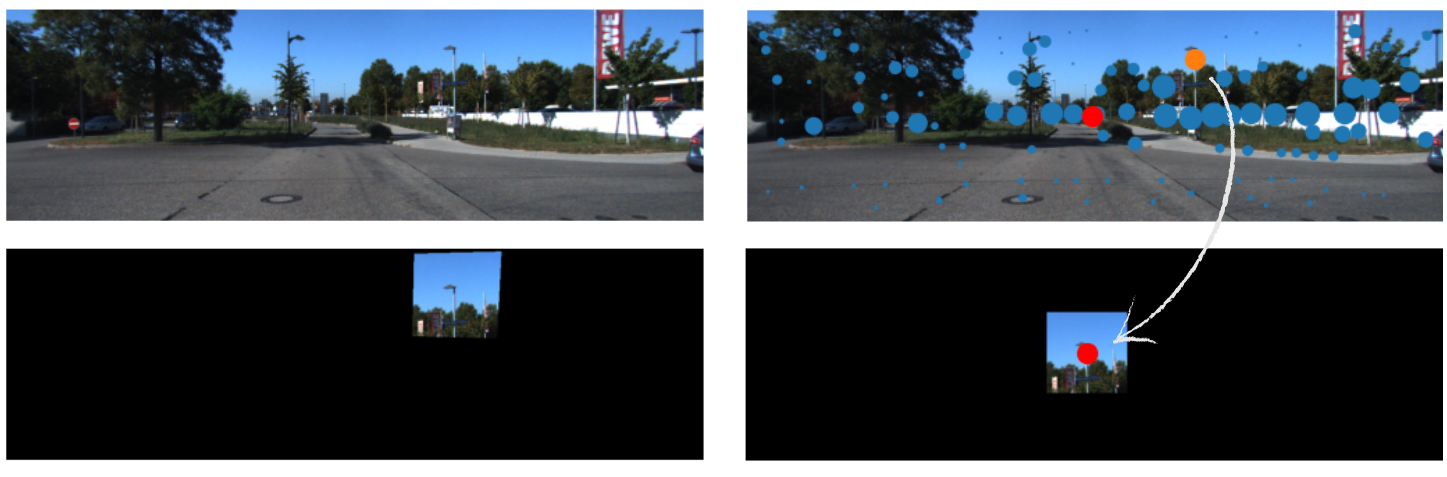
\includegraphics[scale=0.4]{figs/warping}
    \end{adjustwidth}
    \caption{
        The image shows the warping procedure applied to a point sampled with the corner strategy.
        Top-left: the image $\mathbf{I}$ from which to extract patches.
        Top-right: detected corners. The orange point is the selected corner. The red point is the principal point.
        Bottom-right: the warped and cropped image $\tilde{\mathbf{I}}$.
        Bottom-left: the corresponding unwarped region in the original image.
        \label{fig:warping}
    }
\end{figure}
The procedure, illustrated in figure \ref{fig:warping}, is the following:
\begin{enumerate}
    \item{Sample a point $p$ from image $\mathbf{I}$.}
    \item{Compute the camera transformation that maps $p$ to the principal point.}
    \item{Warp the image using the computed transformation and obtain a new image $\tilde{\mathbf{I}}$.}
    \item{Crop $\tilde{\mathbf{I}}$ around the principal point.}
\end{enumerate}
This procedure can produce patches with out-of-view pixels.
To mitigate this, in the sampling procedure, strips along the full-image borders are ignored.
Moreover, the warping can produce lower quality images since a bilinear interpolation step is required.
Instead, for producing the depth map of the patch, the point cloud provided with the image is projected onto the image, coherently with the computed transformation.
This warping procedure simulates patches captured with identical cameras and imitate human eyes that rotate (as the camera here does for warping) for observing different visual regions.

Another consideration is that when building the full image depth map, a lot of partial predictions are stitched together.
Depth estimation on a single patch doesn't need to be perfect if its imperfections can be corrected by the other predictions.
For this reason, a weighted variant of the scale invariant loss introduced by Eigen~et~al.~\cite{Eigen} is employed.
The weighting uses a gaussian density function with standard deviation set to $(w + h) / 2$ and weights pixels based on their distance from the middle point of the patch of coordinates $(h/2, \, w/2)$.
If a pixel $p$ has image coordinates $(i, \, j)$, its weight $w(p)$ is defined as:
\[
    w(p) \, = \, w(i, j) \, = \,
    \text{exp} \Bigl\{
        \frac{
            (i \, - \, \frac{h}{2})^{2} \, + \,
            (j \, - \, \frac{w}{2})^{2}
        }{
            h \, + \, w
        }
    \Bigr\}
\]
Also the metrics from table \ref{t:metrics} are pixel-wise weighted for measuring the performance of the model.

Since the depth prediction is asked to be more precise in the middle of the patch, boundary details could be less relevant for achieving this.
Thus, a radial blur is applied to each patch.
The blur effect is given by iteratively applying Gaussian blurring to the original patch $\mathbf{P} = \mathbf{P}_{0}$, obtaining $\mathbf{P}_{1}, \mathbf{P}_{2}, \dotsc, \mathbf{P}_{N}$.
Each blurred patch is then center-cropped to different sizes.
To the most blurred one $\mathbf{P}_{N}$ no cropping is applied, to $\mathbf{P}_{N-1}$ a center crop slightly smaller than the previous is applied, and so forth iteratively.
The obtained images have various decreasing sizes:
\[
    w = w_{N} \, > \, w_{N-1} \, > \, \dotsc \, w_{1} \, > w_{0} \, > w_{min}
\]\[
    h = h_{N} \, > \, h_{N-1} \, > \, \dotsc \, h_{1} \, > h_{0} \, > h_{min}
\]
Where $w_{min}$ and $h_{min}$ represents the minimum shape of the non-blurred area.
The radially blurred patch is obtained by concentrically overlapping this patches on top of each other, starting from the most blurred one.
This procedure doesn't apply a proper radial blur, but it produces a similar visual effect.
An example of patches transformed using the outlined procedure can be found in figure \ref{fig:blur}.
\begin{figure}
    \begin{adjustwidth}{-0.2\textwidth}{-0.2\textwidth}
    \centering
    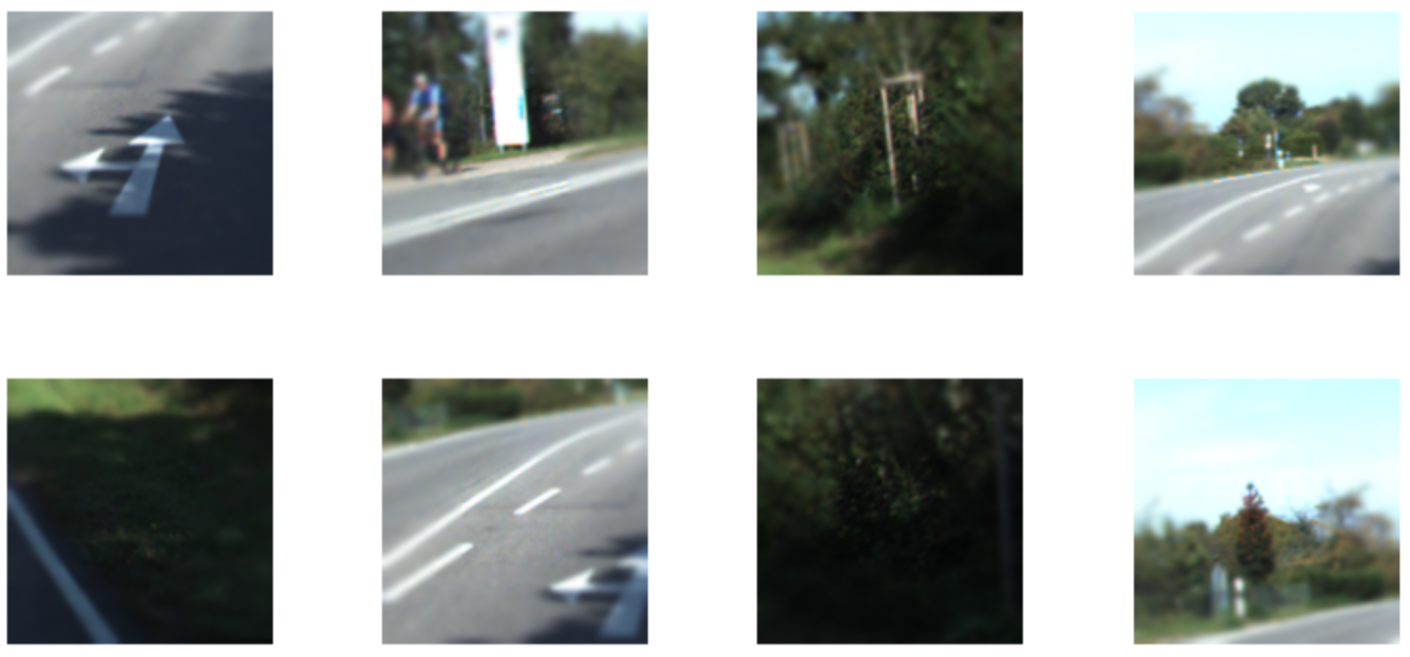
\includegraphics[scale=0.4]{figs/blur}
    \end{adjustwidth}
    \caption{
        Examples of radially blurred patches extracted from an image.
        \label{fig:blur}
    }
\end{figure}
The blurring smooths out the data manifold and reduces its dimensionality.
The informal reason for this is that patches with high-frequency details around the border are mapped to lower-frequency versions, which are less numerous in this finite sampling context.
The new space of radially blurred patches is not a subset of the initial patch space, since the radial blur is not naturally present in considered images.
Whether it simplifies the learning problem or not, is discussed in the next chapter.

\section{Depth fusion pipeline}
\label{sec:depth_fusion}
After having gathered partial depth predictions of the input image, an algorithm for composing a final unique estimation is needed.
Here, a theoretical discussion is made on how such a pipeline could be designed.

The depth fusion part must be as interpretable as possible since a black-box model has been employed for the DE part.
%In the section \ref{sec:miscellaneous}, a tile-based method for DE was discussed: PatchFusion \cite{PatchFusion}.
%While extremely powerful, it is an end-to-end non-interpretable deep learning model that estimates depth patch-wise and subsequently merge them.
% BoostingDepth \cite{BoostingDepth} instead uses a two-stage method with a pre-trained MiDas \cite{MiDas} model for depth estimation and a UNet architecture for merging, but still the overall algorithm is not interpretable.
% The older works from Konrad et al. \cite{konrad2} and Karsch et al. \cite{DepthTransfer}, and a very recent work from Rey-Area et al. \cite{360MonoDepth}, use handcrafted pipelines for the depth fusion part.
% Except for Konrad et al. who take the median of the depth values to be aggregated, the others set up an optimization problem describing desirable properties the resulting full-resolution depth map should satisfy.
I propose to perform a fine-tuning of the black-box model at inference time for merging the estimated patches.
A formulation of the tuning objective is needed, but the knowledge of the network is exploited for making the depth adjustments rather than explicitly parametrizing them (as other works instead do \cite{konrad2, DepthTransfer, 360MonoDepth}).
One could argue that during inference time there is no ground truth available and hence the tuning would be arbitrary.
But, since the model was trained with a loss that put more emphasis on certain areas of the patches, this information could be exploited by treating those areas as ground truth.

The following is inspired by how humans analyze images: they explore them with the eyes building "paths" to follow for visual reasoning and, sometimes, retract their conclusions by exploring the image differently.

\vspace{0.5cm}

Let $\mathbf{I}$ be the input image, $\mathbf{P}_{0}, \mathbf{P}_{1}, \mathbf{P}_{2}, \dotsc, \mathbf{P}_{N}$ the patches and $\mathbf{Z}_{0}, \mathbf{Z}_{1}, \mathbf{Z}_{2}, \dotsc, \mathbf{Z}_{N}$ their estimated depth maps.
A pixel $p \in \mathbf{P}_{n}$ corresponds to a pixel $\hat{p} \in \mathbf{I}$ and, if some overlap occurs, it corresponds also to a pixel $\hat{p}_{m} \in \mathbf{P}_{m}$ for some $m \neq n$.
All the patches are projected onto the image $\mathbf{I}$ so that pixel coordinates live in the same space.
Hence, a same pixel $p \in \mathbf{P}_{n}$ belongs to $\mathbf{I}$ and can also belong to other patches $\mathbf{P}_{m}$.
The black-box DE model is denoted $f$.
A copy of $f$ is used and denoted $\hat{f}$, this will undergo the fine-tuning stage while $f$ is frozen.
Let's call $\hat{\mathbf{Z}}_{0}, \hat{\mathbf{Z}}_{1}, \hat{\mathbf{Z}}_{2}, \dotsc, \hat{\mathbf{Z}}_{N}$ its predictions on the considered patches.

\begin{figure}
    \centering
    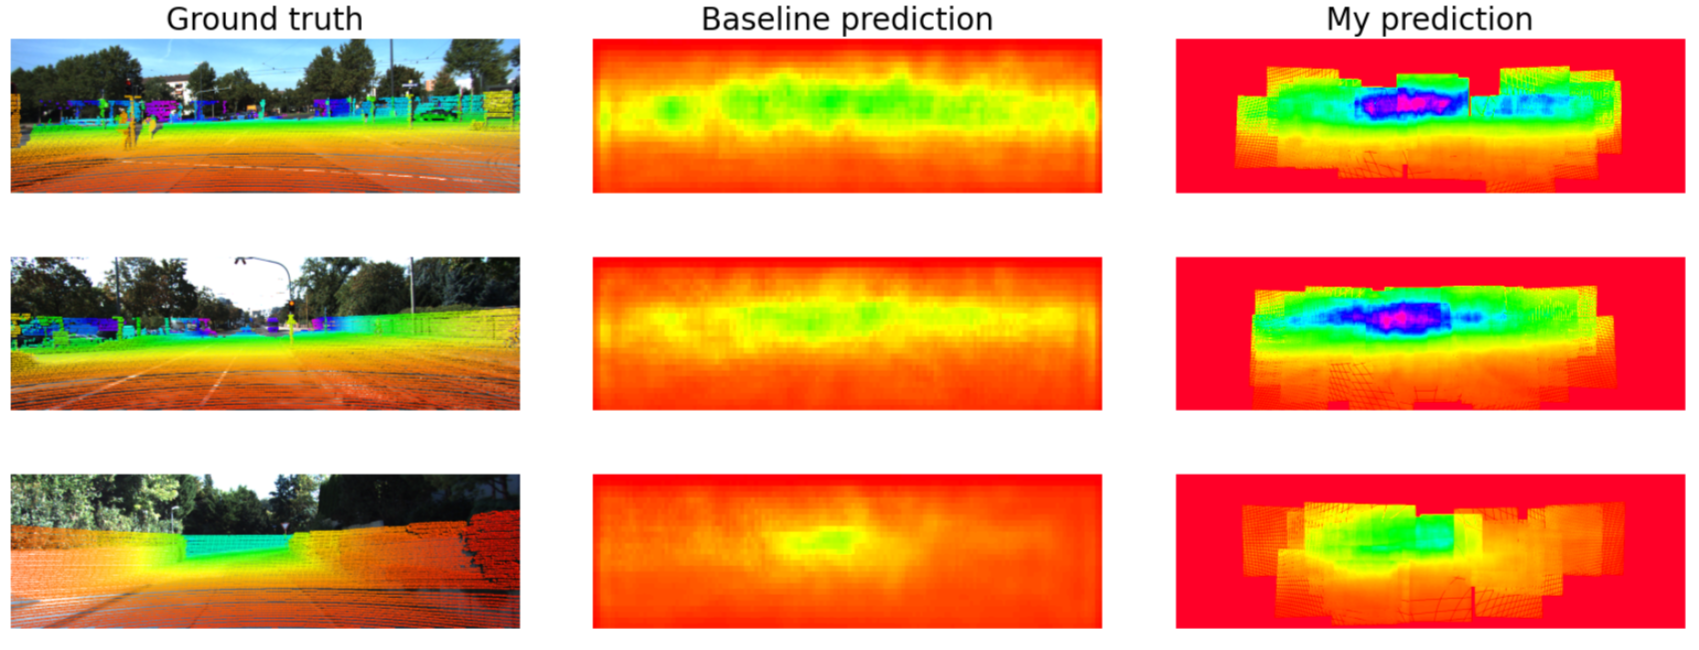
\includegraphics[scale=0.3]{figs/fusion}
    \caption{
        A qualitative example of what could look like the depth fusion pipeline.
        Left: original images from KITTI and their ground truth overlaid.
        Center: predictions from full-image model.
        Right: stitching of partial predictions from patch-model.
        No strategy was developed for dealing with corner-less regions, hence the final result doesn't cover the whole image.
        Visible artifacts are present because of the way differentiable warping was dealt with.
        \label{fig:fusion}
    }
\end{figure}

To make \textit{all} the partial predictions agree on the overlapping regions is a first approach.
The following loss could be minimized:
\[
    \mathcal{L} =
        \sum_{n \neq m} \,
        \sum_{p \in \mathbf{P}_{n} \cap \mathbf{P}_{m}}
        e^{-\mathbf{W}_{n}(p)}
        (\hat{\mathbf{Z}}_{n}(p) - \mathbf{Z}_{m}(p))^{2}
        \, + \,
        \lambda
        \sum_{n}
        \sum_{p \in \mathbf{P}_{n}}
        \mathbf{W}_{n}(p)
        (\hat{\mathbf{Z}}_{n}(p) - \mathbf{Z}_{n}(p))^{2}
\]
Where $\mathbf{W}_{n}$ is a weight mask, as used in the weighted scale-invariant loss and the weighted metrics, that fades radially (if warping was applied to the patch, also the mask is warped).
$\mathbf{W}_{n}(p)$ is a measure of how much the model \textit{should} be confident about the prediction in $p$.
Pixels with high confidence contribute less to the loss.
The first term of the loss encourages different depth maps to agree on the overlapping regions, while the second one avoids the network to completely forget its initial prediction and degenerating into a constant solution. 
As an example, a baseline model was trained on KITTI following \cite{Eigen} and its full-image output was qualitatively compared to a partial depth map obtained with the outlined inference procedure (1 epoch of tuning).
The model used in the inference procedure was trained patch-wise with the various simplifications discussed in the previous section.
During inference, patches are treated analogously.
Figure \ref{fig:fusion} shows the result.

\vspace{0.5cm}

The overlapping between patches need to be monitored since it could create an unbalanced loss.
For this reason, further modifications are required.
Instead of optimizing all patches together, it could be established an ordering.
Also, the model will perform differently on different patches and so not all patches should be treated equally.
A procedure similar to the one used for variable selection in statistics could be employed.
Hence, the optimization would involve an initial small set of patches to which the other ones are iteratively added and optimized, without necessarily using all of them (forward selection).
Or, some could be iteratively removed from the whole set (backward selection).

\begin{figure}
    \centering
    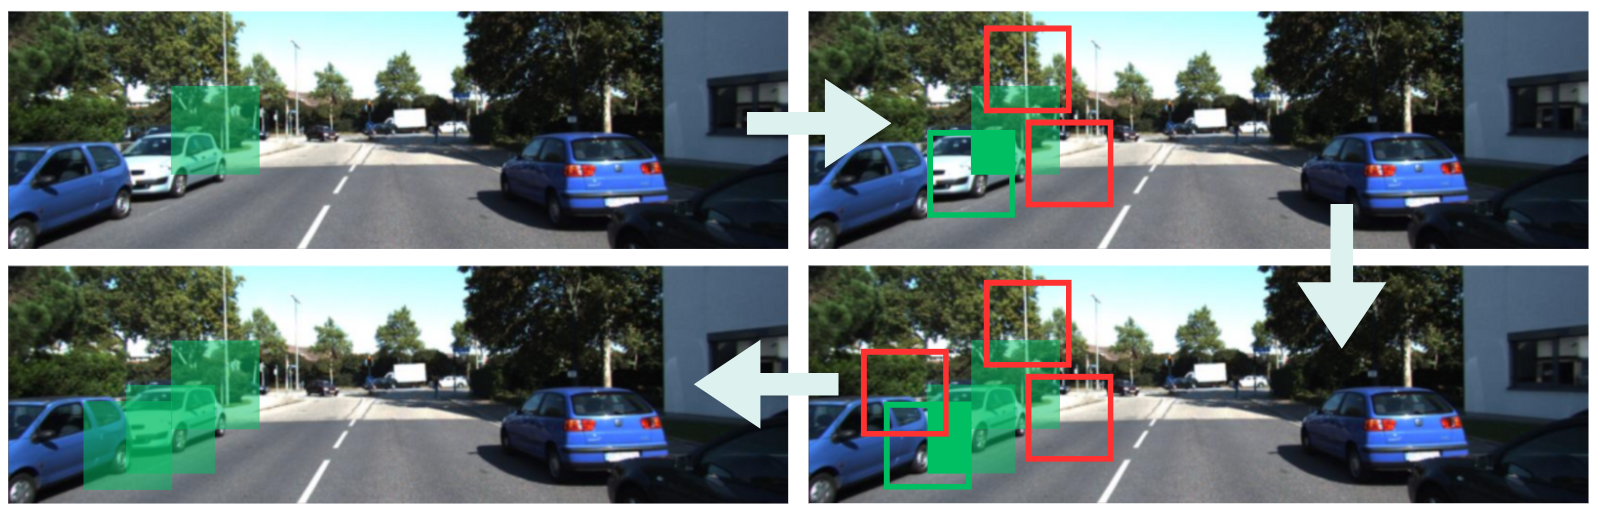
\includegraphics[scale=0.3]{figs/fusion_boxes}
    \caption{
        Top-left: the first patch is chosen and depth is predicted (transparent green).
        Top-right: candidates for the next patch are evaluated, the green box is chosen.
        The solid green rectangle indicates the overlapping region.
        Bottom-right: the process is iterated.
        Bottom-left: it is shown the whole region involved in the prediction up to this iteration.
        \label{fig:fusion_boxes}
    }
\end{figure}


Assume there is a strategy for choosing one or more initial patches in which the model is more confident, i.e. some error measure w.r.t. ground truth is \textit{probably} lower.
For instance, in \cite{BoostingDepth} it is observed that depth estimation models better perform on regions with a precise \textit{edge} density that depends on the dataset the model was trained on.
A simple criterion could be to first select the patch with edge density closest to the reference value.
Let's call $n_{0}$ its index.
Consider now another patch $\mathbf{P}_{n_{1}}$.
If it overlaps with $\mathbf{P}_{n_{0}}$ a comparison can be made and might be used for establishing whether to include it in the optimization process or not.
Ideally, assuming DE is \textit{metric} (otherwise an affine correction is required), patches with a large overlap should agree on depth values, while patches with little overlapping may disagree more.
This is due to the radial weighting applied during training and to a general translational invariance of convolution layers of the black-box\footnote{Their presence is not obvious, but it is extremely common. If they are not present, data augmentation should provide such an invariance.}.
For building a coherent depth map, the second patch must present a compromise between fully overlapping and not overlapping, but it should agree as much as possible with the initial patch.
After the patch is selected it is merged with the previous one, creating a new patch.
If a criterion that fulfills these requirements is defined, it could be used to iteratively add and optimize patches until a condition is met.
A schematic illustration of this iterative inference procedure is found in Figure \ref{fig:fusion_boxes}.

It could happen that some non-optimal choice has been taken during the process.
In this case, a backtracking procedure should be considered for producing an alternative merge.
For successfully applying such a thing, fine-tuned models must be copied each time, producing models $\hat{f}_{0}, \hat{f}_{1}, \dotsc$ corresponding to each iteration of the merging procedure.
This whole fusion pipeline seems computational expensive, but if the neural network used for DE patch-wise is lightweight (and that is the objective of the previous paragraphs) this pipeline is feasible.

%\subsection{Motivations for the proposed pipeline}
%By introspection, I observed the following inner facts about scene depth perception (and reasoning) from single image:
%\begin{enumerate}
%    \item{
%        Depth information of what I am looking at is immediately provided;
%    }
%    \item{
%        When I am looking at something, I am not looking at other things, even if close to it;
%    }
%    \item{
%        The eyes continuously move across the image;
%    }
%    \item{
%        The eyes visit more often ambiguous regions;
%    }
%    \item{
%        Sometimes, the eyes move following precise patterns;
%    }
%    \item{
%        Depth perception of things can change throughout the image analysis;
%    }
%    \item{
%        Explicit visual reasoning is performed using eyes movement;
%    }
%    \item{
%        The eyes tend to look at corners (in the computer vision sense, refer to \cite{computer_vision});
%    }
%    \item{
%        When the eyes look at an edge, they tend to follow it in subsequent movements;
%    }
%    \item{
%        When the eyes look at a texture-less region, they tend to move randomly in it.
%    }
%\end{enumerate}
%The fusion pipeline and experiments formulated above are inspired by these observations.
%The non-interpretable component, in my opinion, must be inserted in the immediate (partial) perception of depth of things (point 1 of the bullet list).
%By things, I don't mean well-formed objects.
%Instead, I refer to places where the eyes stop.
%Point 2 sounds tautological, but it is fundamental.
%It states that when looking at something, even though other things fall into the visual field, no depth information about them is provided.
%Mathematically, it is difficult to express this fact.
%The way I choose to give it a formalization is: the reliability of pixels in an atomic depth estimation decreases radially.
%In this way, for having a reliable depth map of a full image, multiple "looks" at it are necessary.
%This aligns with the tile-based approaches to MDE and with the design choices I made.